% =============================================================================
%  Dinamica3_Fase2_Diapositiva3.tex — Dinámica 3, Fase 2, Diapositiva 3:
%  el lenguaje digerido. Fondo oscuro y limpio; los dos hilos del cap. 34
%  separados y resumidos en lenguaje cotidiano.
%  Resumen de redacción propia, aprobado (3 nov 2026).
%  Formato 16:9. Compilar con: bash ../../../compilar_diapositivas.sh
% =============================================================================
\documentclass[tikz,border=0pt]{standalone}
\usepackage[utf8]{inputenc}
\usepackage[T1]{fontenc}
\usepackage[default]{sourcesanspro}
\frenchspacing   % espaciado uniforme tras punto (convención en español)
\hyphenpenalty=10000 \exhyphenpenalty=10000   % sin división de palabras

% ── Parámetros ────────────────────────────────────────────────────────────────
\def\TamLetra{34}       % tamaño de letra, en pt
\def\Interlinea{46}     % interlineado, en pt
\def\AnchoTexto{25}     % ancho del bloque de texto, en cm

% ── Paleta (Fase 1, Diapositiva 3) ────────────────────────────────────────────
\definecolor{Fondo}{HTML}{141210}
\definecolor{Texto}{HTML}{F3EDE0}
\definecolor{Etiqueta}{HTML}{E8B04B}
\definecolor{Referencia}{HTML}{9C9385}

% ── Dimensiones (16:9) ────────────────────────────────────────────────────────
\def\ancho{32}
\def\alto{18}

\begin{document}
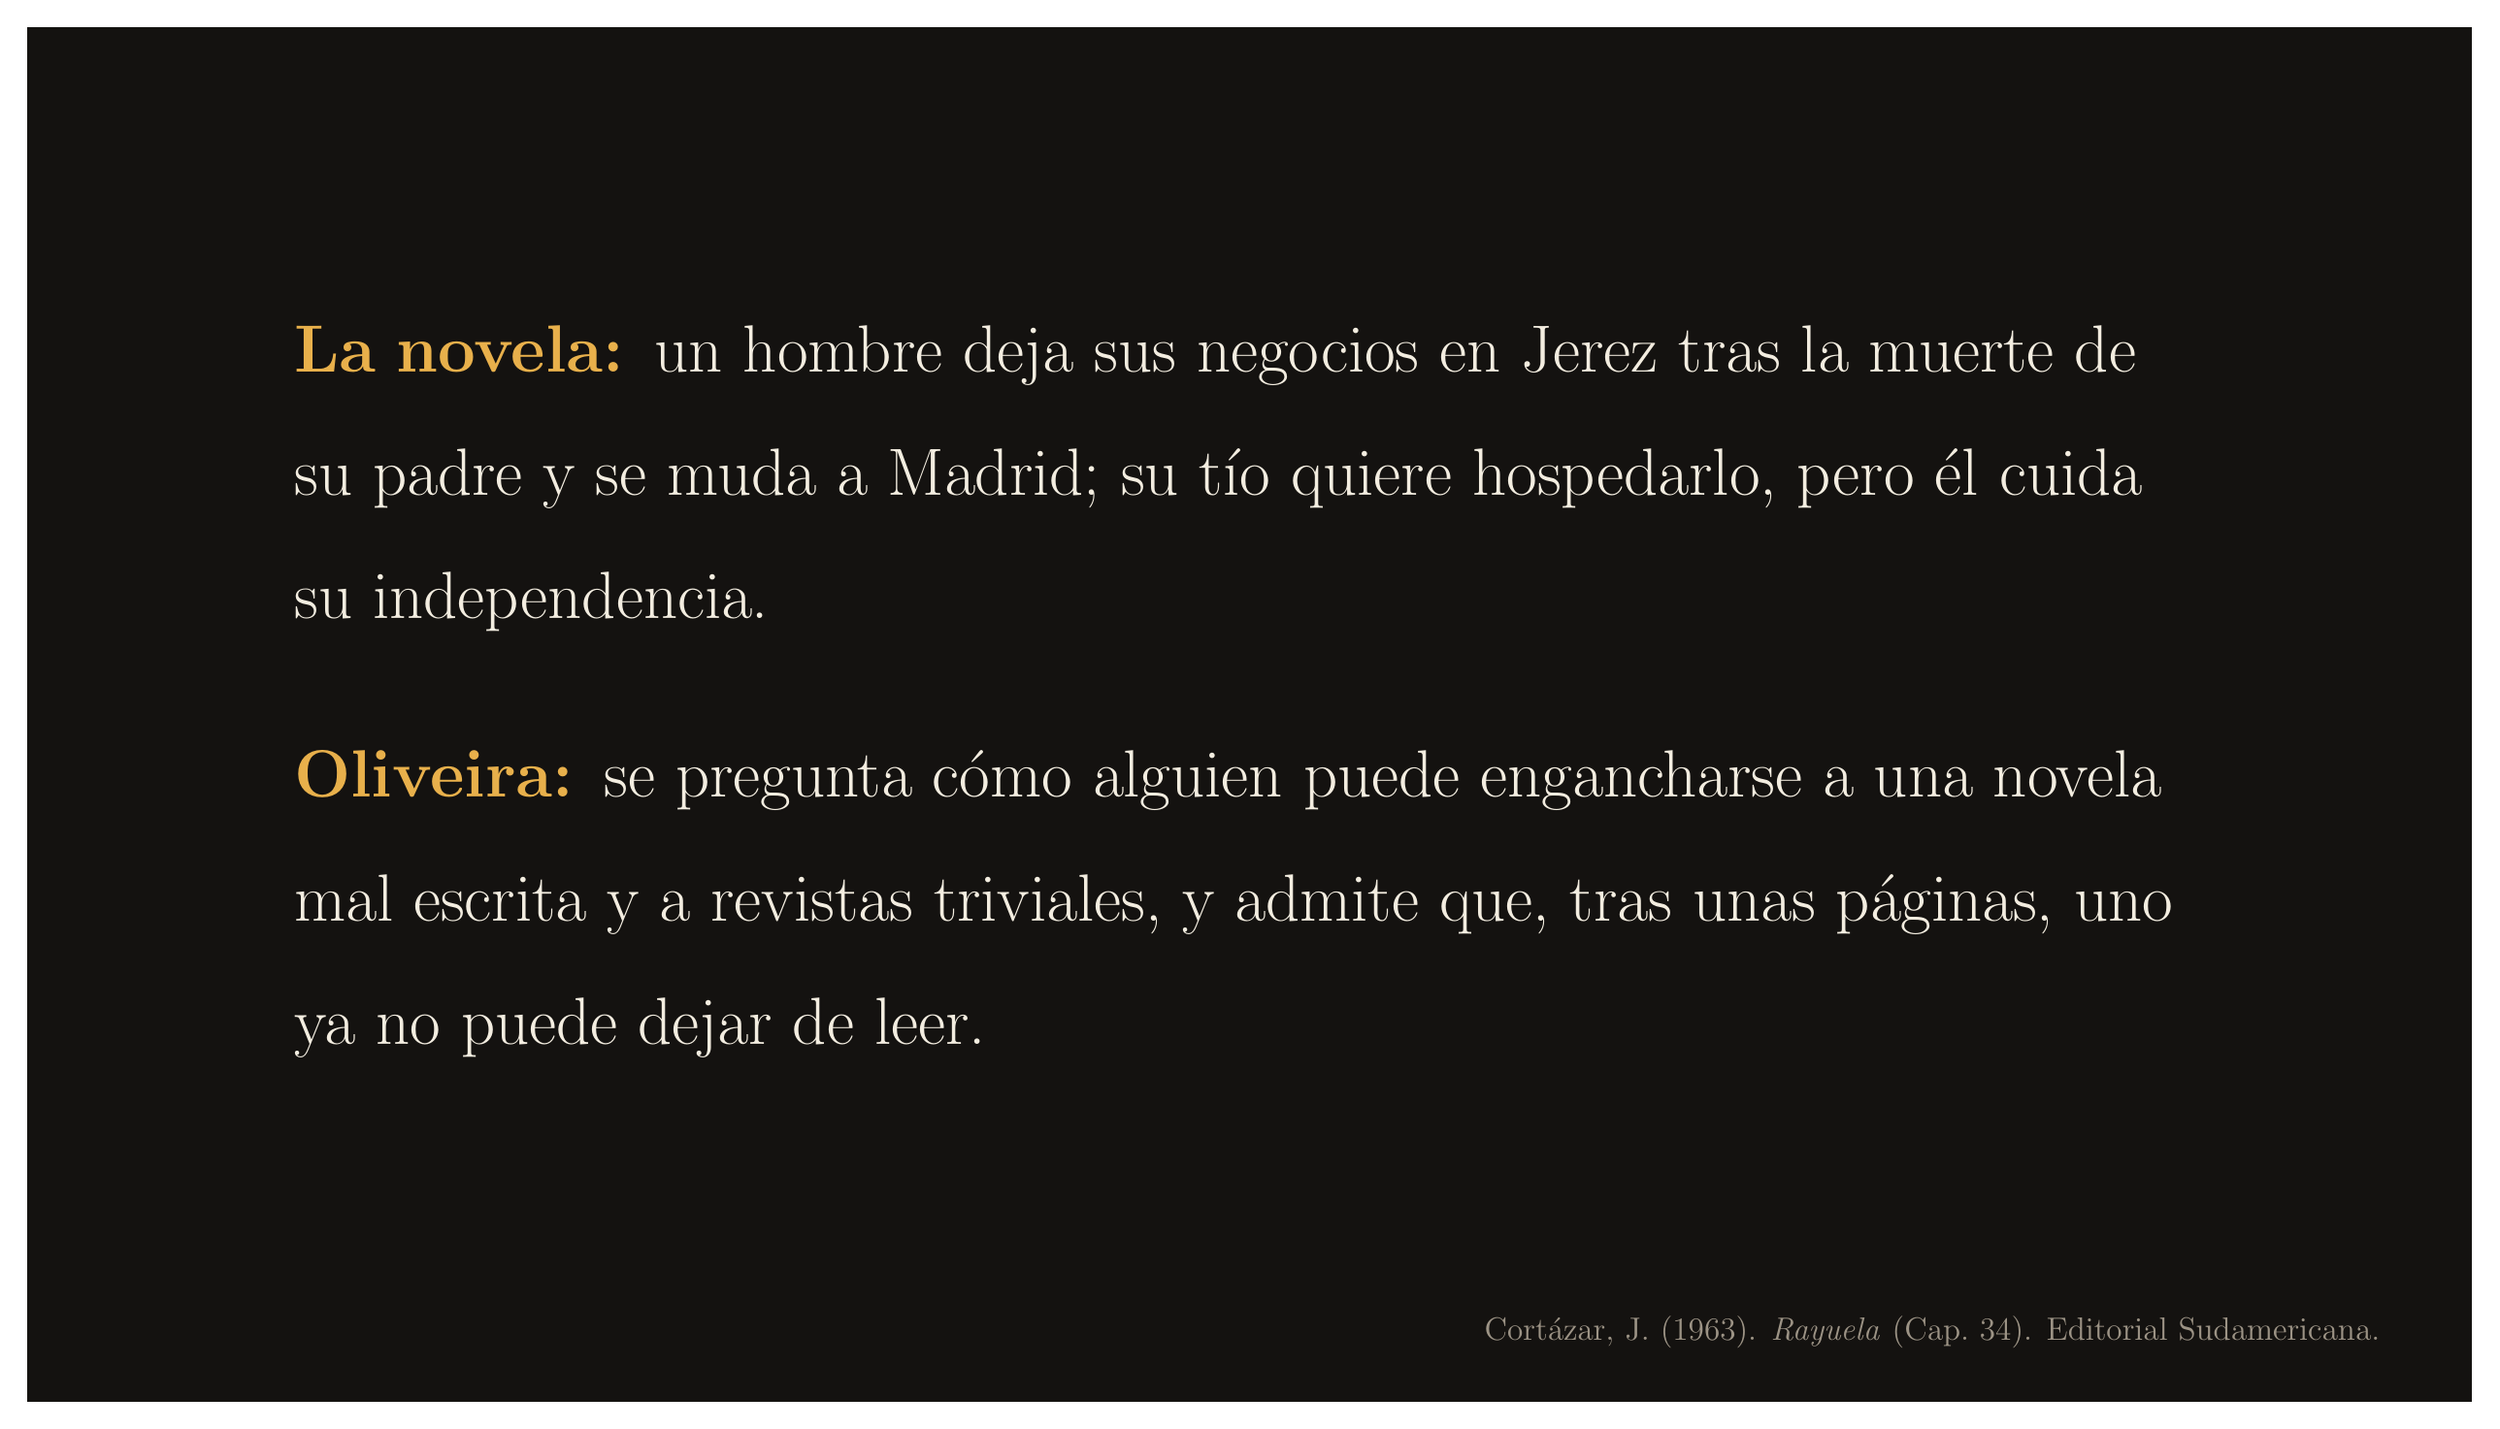
\begin{tikzpicture}
  \useasboundingbox (0,0) rectangle (\ancho,\alto);
  \fill[Fondo] (0,0) rectangle (\ancho,\alto);

  \node[text=Texto, align=left, text width=\AnchoTexto cm,
        font=\fontsize{\TamLetra}{\Interlinea}\selectfont]
    at (\ancho/2,\alto/2+0.3) {%
      {\color{Etiqueta}\bfseries La novela:} un hombre deja sus negocios en
      Jerez tras la muerte de su padre y se muda a Madrid; su tío quiere
      hospedarlo, pero él cuida su independencia.\par\vspace{0.9em}
      {\color{Etiqueta}\bfseries Oliveira:} se pregunta cómo alguien puede
      engancharse a una novela mal escrita y a revistas triviales, y admite
      que, tras unas páginas, uno ya no puede dejar de leer.%
    };

  % Referencia APA
  \node[anchor=south east, text=Referencia, inner sep=0pt,
        font=\fontsize{13}{16}\selectfont]
    at (\ancho-1.2,0.7)
    {Cortázar, J. (1963). \textit{Rayuela} (Cap.~34). Editorial Sudamericana.};
\end{tikzpicture}
\end{document}
